\documentclass[10pt,a4paper]{article}
\usepackage[utf8]{inputenc}
\usepackage[spanish]{babel}
\usepackage{amsmath}
\usepackage{amsfonts}
\usepackage{amssymb}
\usepackage{graphicx}
\usepackage{listings}
\lstset{ frame = single}

\begin{document}

\begin{titlepage}
\title{\textbf{\Huge{Práctica 2}\\
	\large{Seguridad Informática}
}}
\author{
	Pedro Allué Tamargo (758267)
	\and
	Juan José Tambo Tambo (755742)
}
\date{\today}
\clearpage\maketitle
\thispagestyle{empty}
\tableofcontents
\end{titlepage}

\section{Tarea 1: Crear CA}

Se va a proceder a crear una \emph{CA (Certification Authority)}. Para ello se va a crear un certificado y se va a firmar por nosotros mismos. Para ello se va a utilizar la herramienta \texttt{openssl}.\\
Lo primero será obtener una copia del fichero de configuración de \texttt{openssl} disponible en \texttt{/ust/lib/ssl/openssl.cnf}. Se va a modificar el fichero de configuración de tal forma que la variable \texttt{dir} almacene el valor \texttt{./ourCA}.\\
Tras la modificación se van a crear los subdirectorios \texttt{certs, crl\_{}dir, new\_{}certs\_{}dir} y los ficheros \texttt{database} y \texttt{serial}.\\

Ahora se podrá crear el \emph{certificado auto-firmado} para la \emph{CA}. Para ello se ejecutará el comando:

\begin{lstlisting}
openssl req -new -x509 -keyout ca.key -out ca.crt \
	-config openssl.cnf
\end{lstlisting}

La opción \texttt{-x509} indica que el certificado es \emph{auto-firmado}.


\section{Tarea 2: Crear certificado para \emph{seginfo.es}}

Para crear un certificado para \emph{seginfo.es} debemos generar un par de claves públicas/privadas. Para ello utilizaremos el siguiente comando:

\begin{lstlisting}
openssl genrsa -aes128 -out server.key 1024
\end{lstlisting}

El programa pedirá una contraseña para cifrar el fichero \emph{server.key}.\\
Ahora debe ser la entidad certificadora la que firme el certificado. Para ello se debe crear una solicitud de firma de certificado (\emph{CSR}). Para generar el fichero \emph{server.csr} se utilizará el comando:

\begin{lstlisting}
openssl req -new -key server.key -out server.csr \ 
	-config openssl.cnf
\end{lstlisting}

Durante la creación de la petición de firma el programa pedirá datos como el \emph{Common Name}. A este campo se le dará el valor de \emph{seginfo.es}.\\
Una vez obtenido el fichero de petición de firma del certificado se pedirá a la \emph{CA} que firme el certificado. Para ello la \emph{CA} ejecutará el siguiente comando.

\begin{lstlisting}
openssql ca -in server.csr -out server.crt -cert ca.crt \
	-keyfile ca.key -config openssl.cnf
\end{lstlisting}

Ahora el fichero \emph{server.crt} contendrá el certificado firmado por nuestra \emph{CA} que demuestra su identidad frente a la entidad certificadora.


\section{Tarea 3: Implementación de certificados en un servidor web \emph{HTTPS}}

Tras la generación del certificado para el servidor \emph{seginfo.es} se va a proceder a implementar el certificado con un servidor web \emph{HTTPS}. Para este paso se va a realizar una modificación sobre el \emph{DNS} de la máquina para acceder al servidor web de \emph{seginfo.es} (ubicado en la propia máquina). Para ello se modificará el fichero \texttt{/etc/hosts} y se añadirá el siguiente contenido:

\begin{lstlisting}
127.0.0.1 seginfo.es
\end{lstlisting}

Tras la modificación del \emph{DNS} se va a proceder a configurar el servidor web. Para ello ser va a combinar el fichero de clave privada con el certificado en un solo fichero. Para ello se van a ejecutar los siguientes comandos:

\begin{lstlisting}
cp server.key server.pem
cat server.crt >> server.pem
\end{lstlisting}

Tras la combinación de claves procedemos a lanzar el servidor web integrado en la herramienta \emph{openssl} utilizando el comando:

\begin{lstlisting}
openssql s_server -cert server.pem -www
# Si se quiere ejecutar el comando en 
#	segundo plano se utilizara:
# openssl s_server -cert server.pem -www \ 
#	-pass pass:_password_ &
\end{lstlisting}

Si se accede al servidor web utilizando el navegador de la máquina \emph{host}. Para ello se utilizará la IP de la máquina virtual (Figura \ref{fig:tarea3_paso2}). Se puede observar que el navegador no trata a la conexión como segura ya que no dispone del certificado de nuestra \emph{CA}.

\begin{figure}[h!]
\centering
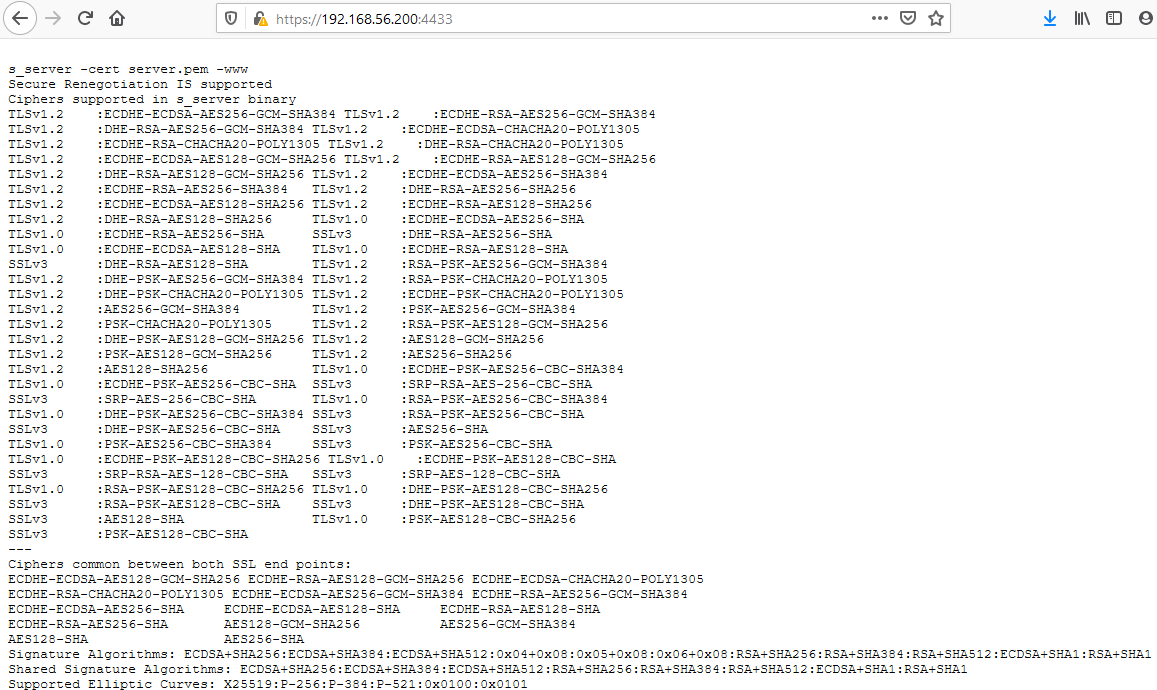
\includegraphics[scale=0.4]{images/tarea3_paso2.png}
\caption{Captura de pantalla del acceso desde el navegador web}
\label{fig:tarea3_paso2}
\end{figure}

Si se intenta acceder utilizando \emph{curl} se obtendrá un error (Figura \textbf{{\LARGE Tambo por favor mete la figura que no tengo la MV}}) ya que no se puede establecer la veracidad del servidor.

% Mete la figura aqui

Para conseguir que \emph{curl} acepte la veracidad del servidor \emph{seginfo.es} se debe añadir un argumento a la llamada:

\begin{lstlisting}
curl --cacert ca.crt https://seginfo.es:4433
\end{lstlisting}

Tras esto se observaría que el resultado es el mostrado en la Figura \ref{fig:tarea3_paso3}.

\begin{figure}[h!]
\centering
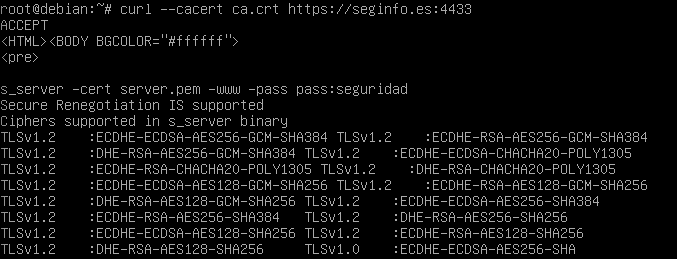
\includegraphics[scale=0.6]{images/tarea3_paso3.png}
\caption{Captura de pantalla del acceso desde curl con certificado de CA}
\label{fig:tarea3_paso3}
\end{figure}


¿Qué pasaría si modificasemos un solo byte del fichero \emph{server.pem}? Depende. Si se modifica un byte de la zona \emph{Certificate} el servidor no se inicia (\textbf{METER CAPTURA DE PANTALLA}). Si se modifica un byte de la zona \emph{signature-algorithm} el servidor se inicia sin problemas (\textbf{METER CAPTURA DE PANTALLA PERO ME EXTRAÑA QUE NO DE NINGÚN ERROR}).

¿Qué ocurre si nos intentamos conectar mediante \texttt{https://localhost:4433}? Que no podremos conectar ya que el certificado ha sido emitido para \emph{seginfo.es} y no para \emph{localhost}.


\section{Tarea 4: Implementación de certificados en un servidor web \emph{HTTPS} basado en \emph{Apache}}


Configurar el servidor Apache2. Modificar ficheros 000-default y default-ssl.\\
Crear directorio \texttt{/var/www/seginfo.es} y fichero index.html (y poner el contenido que le hemos metido).\\
Hacer los comandos de apache2. Introducir el passphrase de la clave al reiniciar.\\
Hacer comando \texttt{curl --cacert ca.crt https://seginfo.es} y decir que sale todo bien.\\

\textbf{Hay capturas de pantalla}


\section{Tarea 5: Lanzando un ataque \emph{MITM}}

Explicar cual es la página a suplantar (example.com).\\
Crear certificado para el sitio que queremos suplantar.\\
Para lanzar un MITM hay que modificar el DNS del host. Explicar como lo has hecho en Windows.\\
Utilizando el navegador web del host ir a example.com.\\
Añadimos el certificado al navegador (firefox) y volvemos a entrar.\\

\textbf{Hay capturas de pantalla}

\section{Tarea 6: Lanzando un ataque \emph{MITM} con una CA comprometida}

Aqui ya no tengo nada apuntado pero yo diría que el atacante ha obtenido la clave privada de la CA y puede firmar lo que quiera. Va a suplantar webs mediante ataque a DNS y ha suplantado la página de www.pcbox.com. Explicar un poco qué ha hecho apoyándote en las tareas 4 y 5.\\

\textbf{Hay captura de pantalla}


\end{document}